\chapter*{Introduction}
\label{Introduction}
\addcontentsline{toc}{chapter}{\textbf{Introduction}}
Humanity is amidst a critical ecological era, whereby the ecological thresholds of the earth system have been crossed. The notion of \textit{planetary boundaries} \citep{rockstrom2009safe,steffen_2015_planetary} illustrates how the anthroposphere, the planetary-scale effects of human activities, have become an additional functional component and are capable of changing the Earth system \citep{richardson_earth_2023} alongside the geopshere (energy flow and nonliving materials in Earth and atmosphere) and biosphere (all living organisms/ecosystems). The "planetary boundaries" framework identifies the limits to the impact of the anthroposphere on the Earth system that can safeguard Earth's interglacial state - the only one where civilization is known - by identifying a "safe operating space". The boundaries concern biosphere integrity, climate change, novel entities (e.g. man-made introduction to the Earth system such as chemical and material pollutants), stratospheric ozone depletion, atmospheric aerosol loading, ocean acidication, biogeochemical flows, freshwater change and land system change. Among these nine boundaries, \cite{richardson_earth_2023} estimate that 6 have been crossed, threatening the stability and resilience of the Earth system. 

\begin{figure}[H]
	\centering
	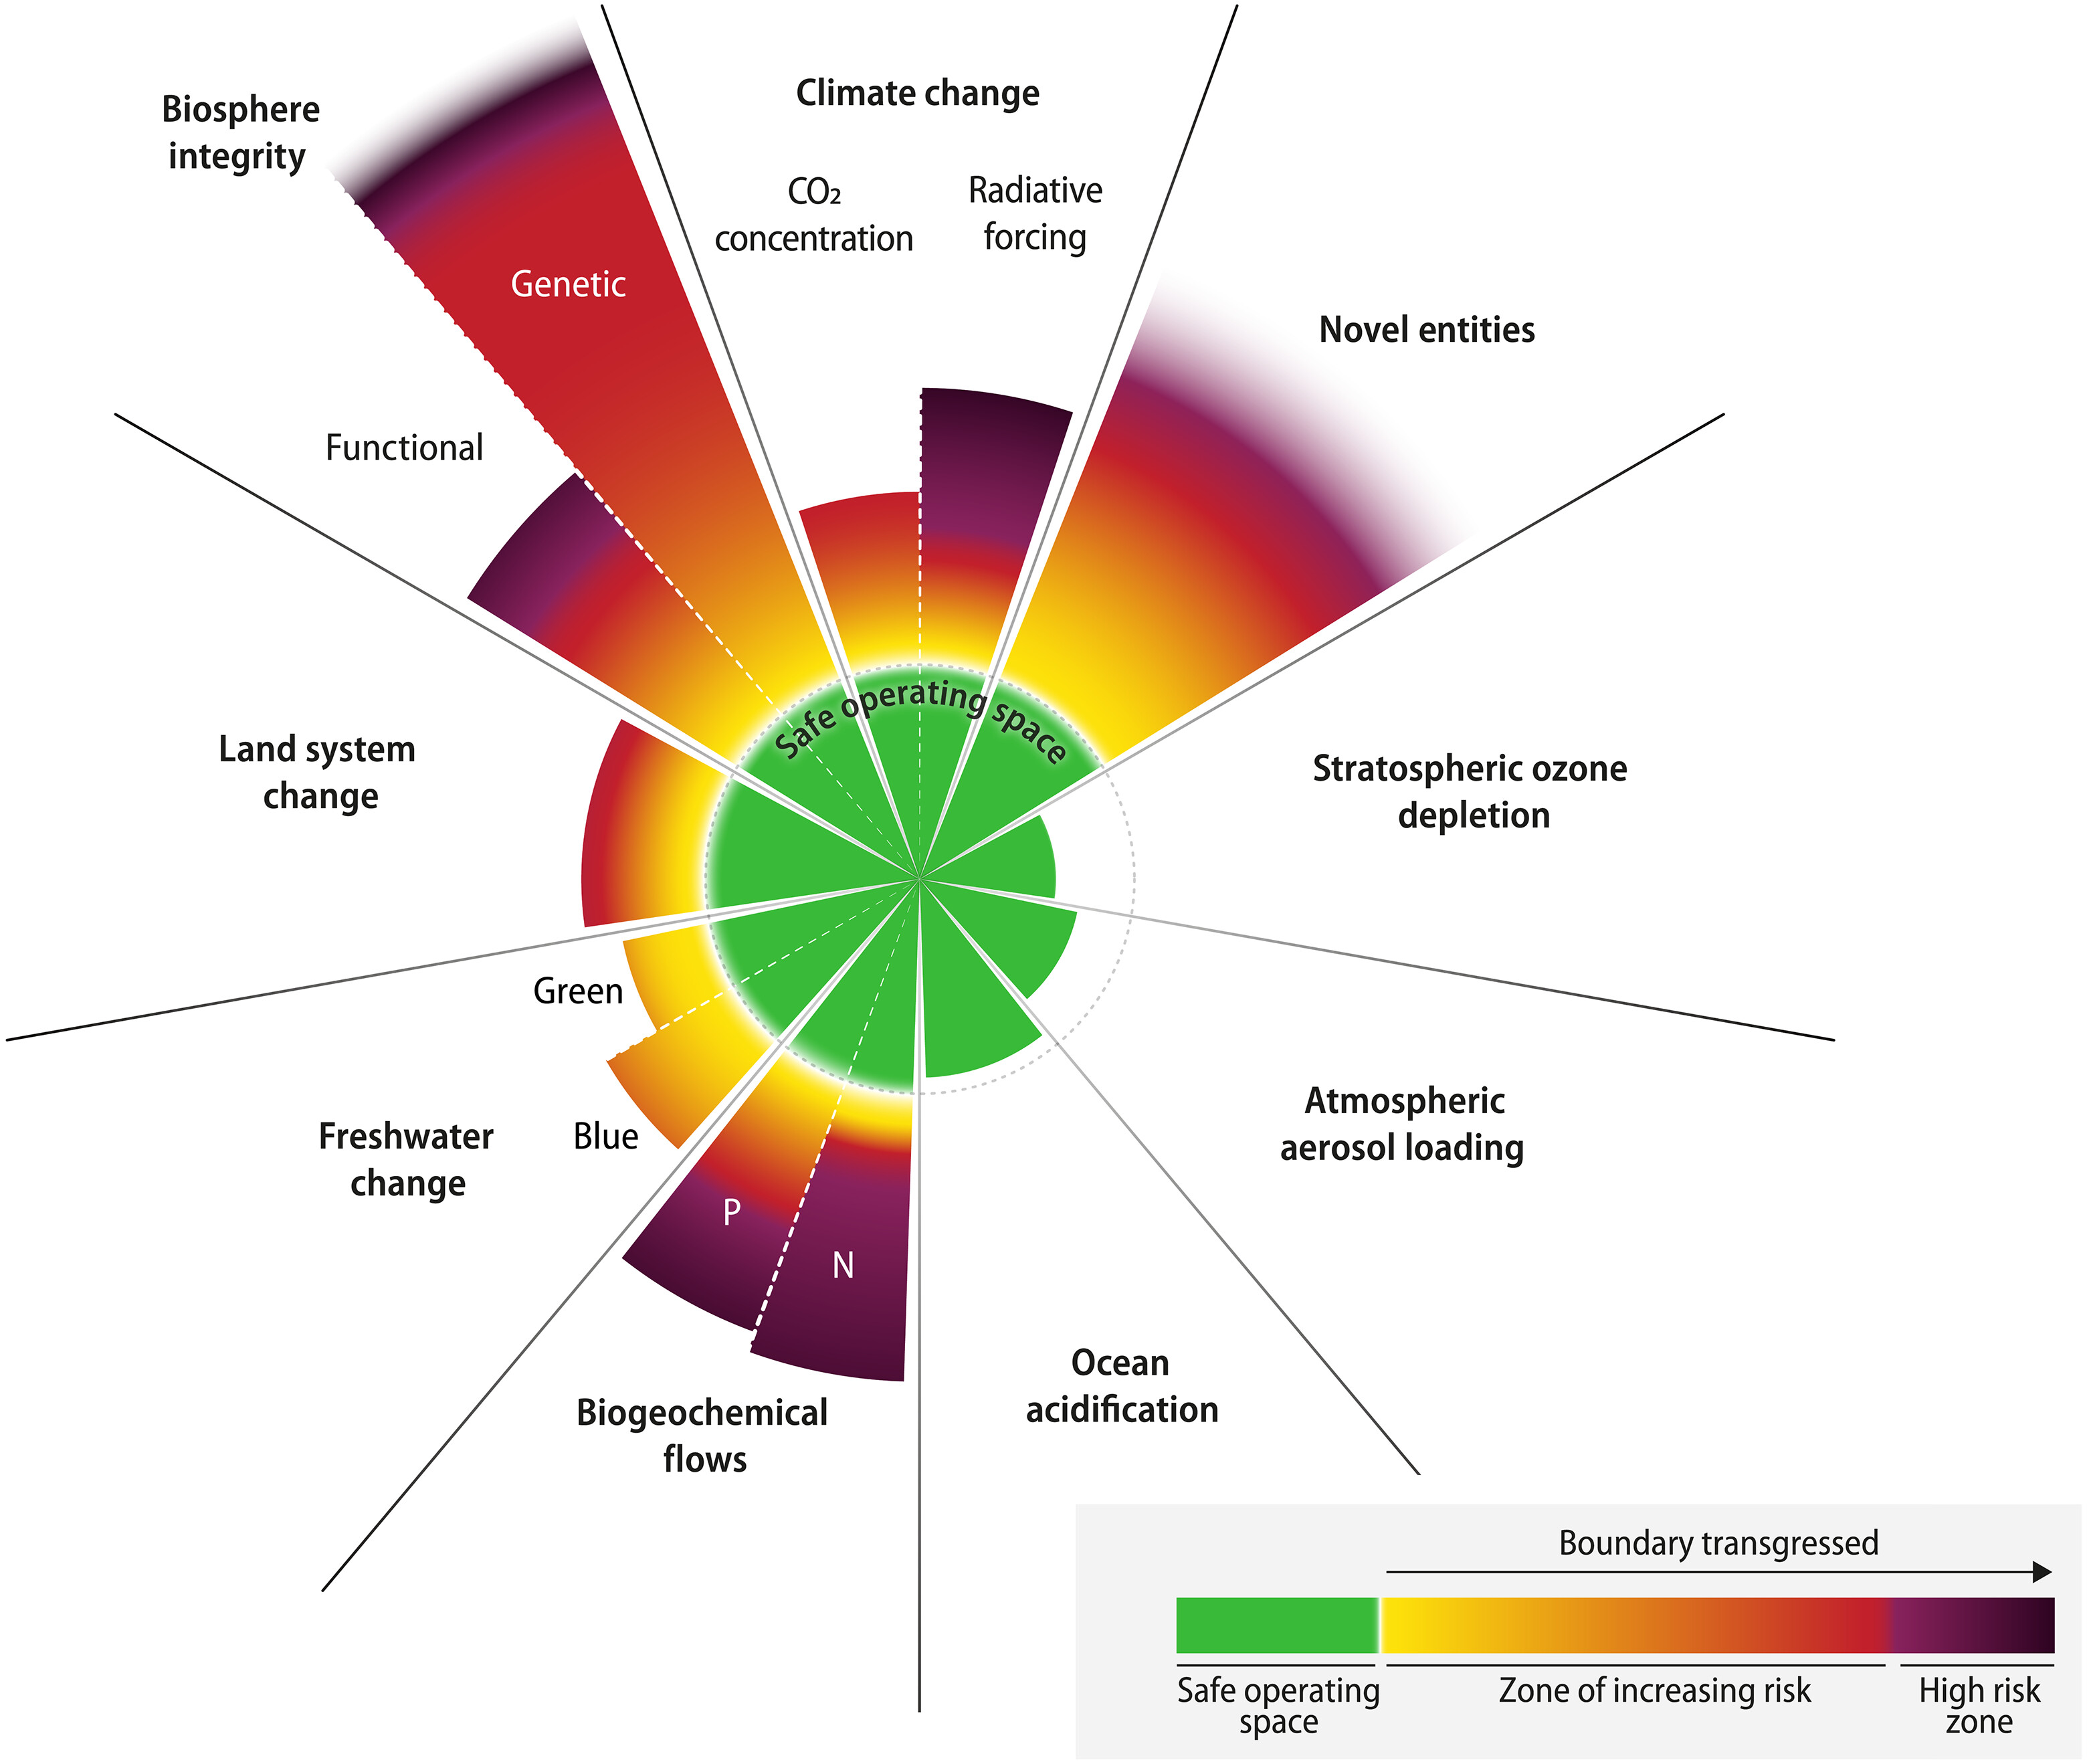
\includegraphics[width= .7\textwidth]{figures/intro/planetary_bounds.jpg}
	\caption{Current status of control variables for all nine planetary boundaries, from \cite{richardson_earth_2023}}
\end{figure}

Among these planetary limits, the integrity of the biosphere has gradually become of particular interest, along with its interaction with other limits, such as climate change, or novel entities (including pollution). Created in 2012, the Interdisciplinary Panel on Biodiversity and Ecosystem Services (IPBES) has been raising the alarm on the state of "Nature" globally. Its chair, Sir Robert Watson, put it clearly\footnote{See the \href{https://www.ipbes.net/news/Media-Release-Global-Assessment}{press release address of the 2019 report}}:
\begin{displayquote}
"\textit{The overwhelming evidence of the \cite{ipbes_2022_6417333} Global Assessment from a wide range of different fields of knowledge, presents an ominous picture [...]. The health of ecosystems on which we and other species depend is deterioriating more rapidly than ever. We are eroding the foundations of our economies, livelihoods, food security, health and quality of life worldwide}"
\end{displayquote}

"Nature" is a central concept in the IPBES framework \citep{ipbes_2022_6417333}:

\begin{displayquote}
\textit{Nature (also defined as living nature) [is] the nonhuman world, including coproduced features, with particular emphasis on living organisms, their diversity, their interactions among themselves, and with their abiotic environment. Within the framing of natural sciences, nature includes e.g. all dimensions of biodiversity, species, genotypes, populations, ecosystems, the biosphere, ecosystem functioning, communities, biomes, Earth life support's systems and their asosicated ecological, evolutionary, biogeochemical processes and biocultural diversity. Within the framework of economics, it includes categories such as biotic natural resources, natural capital, and natural assets. Within a wider context of social sciences and humanities and interdisciplinary environmental sciences, it is referred to with categories such as natural heritage, living environment, or the nonhuman. Within the context of other knowledge systems, it includes categories such as Mother Earth [...], Pachammama [...]}\\
\hspace*{\fill} \small{\cite{ipbes_2022_6417333}, p.14, see also \cite{DIAZ20151}}
\end{displayquote}

Nature, as defined in this approach, is a very large and complex object.
It is defined across ontological and epistemological differences (living and non-living e.g. matter), different types of interactions, at various scales (genotypes v. ecosystems), at different types of processes (biological v. ecological), and across different fields of inquiry (natural sciences v. social sciences). In this dissertation, I study more specifically "biodiversity", which focuses on the variability among living organisms. While it is itself an ambiguous concept, biodiversity tends to put the focus on living organisms, in relation to their material, biotic and abiotic environment (as opposed to the study of the non-living environment) and on its critical role among other components of the Earth system.

The \cite{ipbes_2022_6417333} report focuses on four key elements. First, it documents the drastic changes the biosphere is going through and how Nature and more specifically, biodiversity  are changing, across scales, time and geographic areas. Second, it mainly considers these changes through an \textit{anthropocentric} lense, e.g. mediating the aforementioned changes through the multiple and diverse contributions that Nature and biodiversity bring to people and how their disruption impacts human lives. Third, it highlights the role of anthropogenic (e.g. of human origin) drivers of the disruption of Nature and biodiversity. Finally, they underpin ``our economies, livelihoods, food security health and qualitify of life worldwide", the synthesis of the available science calls for collective action and suggests policy pathways to remedy the demise of Nature and biodiversity. 
 
This reports sets different objectives to scientific research. The first objective is to explain the feedback mechanisms : how do human livelihoods impact biodiversity? In response, how does biodiversity impact human livelihoods? This objective involves understanding the causes and measuring the direct and indirect anthropogenic drivers of change in Nature and biodiversity on the one hand, and on the other hand understanding the channels and scales through which Nature and biodiversity contribute to human livelihoods, as well as measuring these contributions. Hence, studying the demise of nature, and the potential to remedy it calls for an integrated perspective, that joins natural sciences to social sciences, through frameworks such as social-ecological systems \citep{Ostrom2009}. 
\\
The second objective is to provide a framework to assess the desirability, the feasibility and means of implementation of collective pathways that would remedy the crisis Nature is facing. In a way, it involves designing and implementing policy pathways towards sustainable futures, e.g. finding definite courses or methods of action selected from alternatives, at the individual, collective or governmental levels, to achieve future states of the world which remain in a safe operating space regarding planetary bounds \citep{rockstrom2009safe,steffen_2015_planetary}.

In this dissertation, I take on these two objectives using a framework stemming from economics and ecology. A first version of the research questions this thesis aims at solving is: 
\begin{enumerate}
\setlength{\itemsep}{0pt} % No space between items
\item What are the feedback relationships between biodiversity and antropogenic drivers of its decline? 
\item What underlying mechanisms must policy pathways tackle to remedy this demise?
\item  How can integrated economic and ecological approaches be used and refined to analyze inform and design policies? 
\end{enumerate}

In order to refine these questions, I first define the concept of biodiversity, through its natural and social sciences appraisals, and highlight ongoing trends in its demise.


\subsection*{The decline of biodiversity : definition and trends}
\addcontentsline{toc}{section}{The decline of biodiversity : definitions and trends}

"Biodiversity" is also an ambiguous, multiform concept from scientific ecology, measurable at different scales and historically charged with agency (e.g. with a mission). Recent data show that it is unambiguously declining. 

\subsection*{Emergence and definition of biodiversity as an ecological concept}
\addcontentsline{toc}{section}{Emergence and definition of biodiversity as an ecological concept}

Biodiversity emerged as a concept in the 1980s, along with the emergence of "conservation biology", a branch of biology concerned with the protection of "biological diversity" \citep{soule_what_1985}, as a response to an acceleration in the loss of species, which have intrinsic value, e.g. should be protected for their own sake \citep{soule_conservation_1986}. 
The concept of biodiversity is therefore embedded in an ethical judgement and a call for action. In the wake of the 1992 Rio United Conference on Environment and Development, the Convention on Biological Diversity emerged as an international treaty to safeguard biodiversity. In doing so, it provided an internationally agreed upon definition:

\begin{displayquote}
"\textit{"Biological diversity" means the variability among living organisms from all sources including, inter alia, terrestrial, marine and other aquatic ecosystems and the ecological complexes of which they are part; this includes diversity within species, between species and of ecosystems.}"\\
\hspace*{\fill} \small{\href{https://www.cbd.int/convention/articles/default.shtml?a=cbd-02}{Article 2 of the Convention on Biological Diversity}}
\end{displayquote}

This definition highlights a key differentiating feature from other parts of Nature, e.g. the living nature of the objects of study. Compared to abiotic factors, biological diversity is characterized by intrinsic growth and reproduction rates (at the individual and population levels), and evolution (at the genetic, and species level). Additionally, these rates of change through time are commensurable with human experience, and most processes (e.g. reproduction, population collapse or recovery, genetic evolution) can be observed within a human lifetime as opposed to the geological temporal scale. 

As highlighted by \cite{mouysset_diversity_2023} and \cite{VanDyke2008}, the definition of biodiversity is difficult, as it recovers ethical, conceptual and measurement dimensions. Biodiversity can be viewed as "an intrinsic, value-ladden quality of natural systems that should be preserved for its own sake" \citep{VanDyke2008, mouysset_diversity_2023}, but it also refers to measurable features
% relevant to understanding genetic distribution, population levels, community structure (e.g assembly of interacting species in a given area), environmental processes, and ecosystem functions (e.g. the ecological processes performed by living organisms, such as carbon sequestration, nutrient recycling, water filtration etc). 

Following \cite{mouysset_diversity_2023}, this definition implies different scales from a hierarchical perspective, at the genetic level, at the species, the community, and the ecosystem levels (defined as the interaction of communities and their abiotic environment). These levels imply different forms of measurement, including the distribution of genes, species abundance (e.g. the number of individuals in a population, at a given time and location), species richness (e.g. the number of different species, at a given time and location) within communities, among communities, and across larger scales (e.g. alpha, beta and gamma diversities.), as well as variations in the abiotic factors that form ecosystems, such as temperature, humidity, water quality, soil quality etc. 
\\
It also comprises different types of diversity : structural diversity (for example, the layers of canopy in forests, the sex-ratio in animal populations), compositional diversity (the variety and abundance of species within a community), and functional diversity (variety of environmental processes performed by living organisms in a given area e.g. carbon sequestration, nutrient cycling or seed dispersal, see \cite{loreau_biodiversity_2002})

\begin{figure}
	\centering
	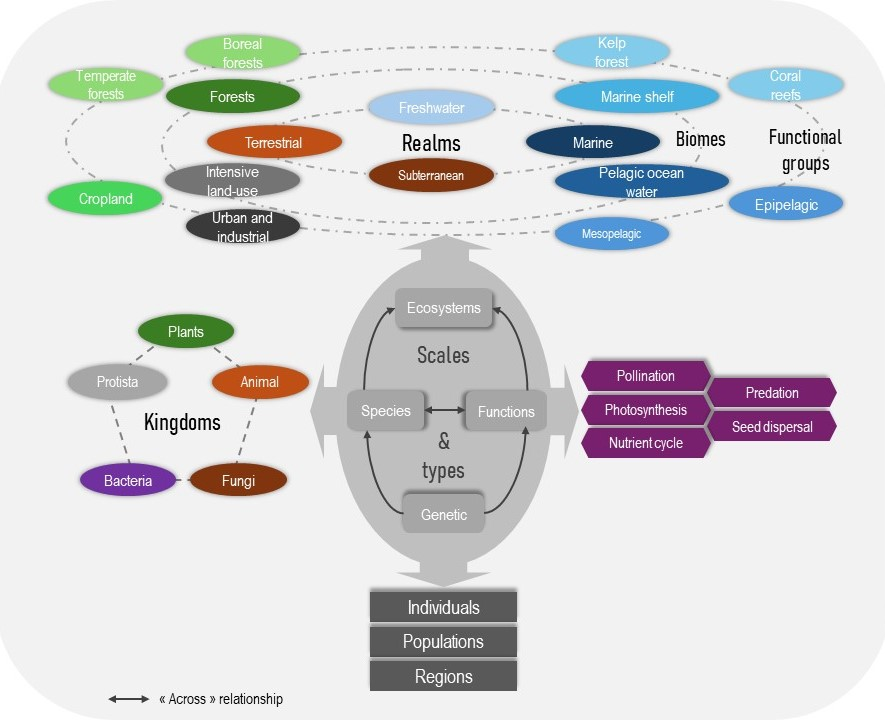
\includegraphics[width =.8\textwidth]{figures/intro/biodiv_illustration.jpg}
	\caption{Biodiversity : a multiform concept across scales and types}
	\label{fig:intro_biod}
\end{figure}

The multiple dimensions of biodiversity highlight several of its critical features. First, it is impossible to measure biodiversity with a single indicator. The study of biodiversity requires multiple indicators to integrally assess the evolution of biodiversity, across scales and types of diversity. The concept and its measurements imply value judgements that shape action. Across all scales, recent data unambiguously show a stark decline in biodiversity. 

\subsection*{Documenting the decline through different scales and biomes}
\addcontentsline{toc}{section}{Documenting the decline through different scales and biomes}

There has been an ongoing decline in metrics of biodiversity. Across all the scales of analysis, the state of nature is critical. The structural conditions of ecosystems (e.g. interactions between biotic and abiotic elements that cause different structural phenomena and lead ecosystems to provide various resources, including wildlife habitat, carbon sequestration etc), the compositions of ecological communities (e.g. species richness) and populations of species (e.g. species abundance) have experienced dramatic changes. 

Ecosystem structure e.g. the arrangement of biotic and abiotic elements through time and space, forms the basis of natural and social-ecological processes. Ecosystems can be classified among realms (terrestrial, subterranean, marine, freshwater etc), biomes (e.g. forests, intensive land uses, marine shelf, pelagic ocean water) and functional groups (temperate forests, cropland, coral reefs, etc) (see figure \ref{fig:intro_biod}). Ecosystem characteristics are severely degraded: only 13\% of oceans and 23\% of land remains sufficiently unimpacted by humanity to be classified as \textit{wilderness} \citep{watson_2016_catastrophic, jones_2018_location}. e.g. areas with "a large area of unmodified or slightly modified land and/or sea, retaining its natural character and influence, which is protected and managed so as to preserve its natural condition" \citep{dudley2008guidelines}.
 On land, at a more refined scale, while deforestation has slowed since the 1990s, vegetation biomass (including trees) has dropped to below 50\% of the level expected absent human land-use, suggesting that a planetary boundary has been crossed \citep{steffen_2015_planetary}. Additionally, anthropogenic climate change drives ecosystem disruptions on land \citep{burrell_anthropogenic_2020, conradi_reassessment_2024} and at sea \citep{gomes_marine_2024}, through changes in various channels including ecological suitability and foodweb disturbances.

Community compositions are changing rapidly, but the average effect remains unclear, as the introduction of alien, disturbance-tolerant, climate-migrant species faces local extinctions is spatially hetorogeneous \citep{cardinale_local_2018}. Analysis from long series of spatial data show contrasted results, because of geographic biases, on land and at sea \citep{dornelas_assemblage_2014, gonzales_estimating_2016}. When taking a historical reference point, however, the fraction of originally present biodiversity falls well below 90\% across all biomes \citep{Hill311787} and local communities are becoming more and more similar \citep{mckinney_1999_biotic}, driven by the increased extent of animal and plant non-alien invasive species, rising by 13\% per decade \citep{seebens_no_2017}. On aggregate, species richness per grid cell is difficult to measure, as slight decreases measured since 1970 \citep{Kim300632} do not account for species introduction, nor potentially unredeemed extinction debts (see below) \citep{JACKSON2010153}.

Finally, at the species level, global species richness is threatened by a mass extinction, as the global rate of species extinction is at least ten times higher than the average rate over the past 10 million years and is accelerating \citep{barnosky_has_2011, ceballos_accelerated_2015}. On average, 25\% of species are currently threatened with global extinction (Figure \ref{fig:intro_iucn}, \cite{IUCN_redlist_2024}) across a wide range of plant and animal species, on land and at sea. Using different methods\footnote{ The IUCN Redlist uses detailed accounts for species, in a bottom-up approach, to analyze the extinction risk of species. A top-down approach, relying on the evolution of available habitat and the species-area relationship, uses changes in land use to forecast the extinction of species in a more aggregate manner \citep{Diamond1972BiogeographicKE}}, \cite{Hoskins309377} find that hundreds of thousands of plant and animal species are threatened, and will repay the \textit{extinction debt} caused by anthropogenic changes to their habitats : only 92.1\% of terrestrial vertebrate species, 91.6\% of terrestiral invertebrates and 90.7\% of terrestrial plants have enough habitat to persist. These results suggest that around half a million terrestrial animal and plant species - including over 3000 vertebrates and over 40,000 plants - \textit{dead species walking}, doomed to become extinct, unless their habitats improve in time to prevent it \citep{ipbes_2022_6417333}.

\begin{figure}[h]
    \centering
    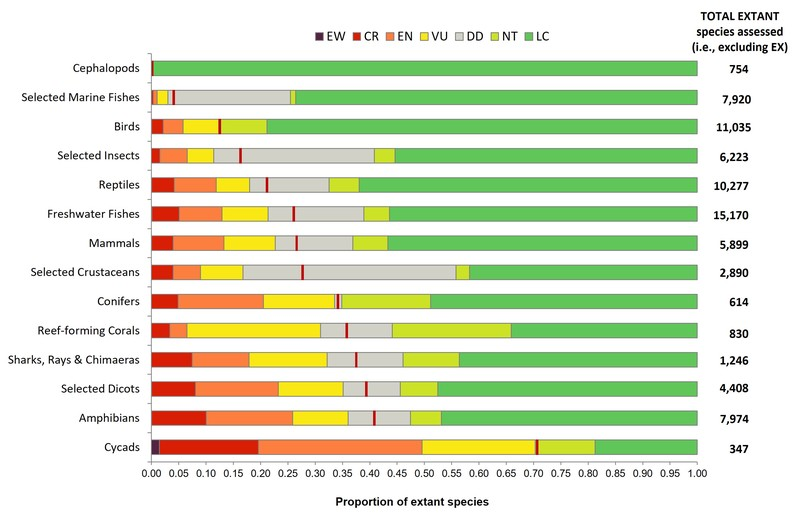
\includegraphics[width=0.8\linewidth]{figures/intro/IUCN_redlist}
    \caption{The proportion of extant (i.e., excluding Extinct) species in \citet{IUCN_redlist_2024}}
    \subcaption*{Assessed in each category for the more comprehensively assessed (i.e., at least 80\% of the group has been assessed) groups containing $\geq$ 150 species. Species are grouped into classes. The numbers to the right of each bar represent the total number of extant species assessed for each group. \textbf{EW} - Extinct in the Wild, \textbf{CR} - Critically Endangered,\textbf{ EN} - Endangered, \textbf{VU} - Vulnerable, \textbf{NT} - Near Threatened, \textbf{DD} - Data Deficient, \textbf{LC} - Least Concern.}
    \label{fig:intro_iucn}
\end{figure}
  
The concept of biodiversity was forged to highlight the need to safeguard the diversity of living organisms across scales from an extinction crisis. Although it arguably was to preserve biodiversity for its own sake, the concept has gradually gained policy power. If biodiversity decline is a policy issue, it is because it underlies Nature's Contributions to People \citep{DIAZ20151}.

\subsection*{Nature's Contributions to People: rationales for biodiversity conservation}
\addcontentsline{toc}{section}{Nature's Contributions to People: rationales for biodiversity conservation}

Biodiversity can be defined at various scales and across different types, but also in terms of the value it bears. As expressed earlier, the coining of the phrase "biodiversity" is intrinsically linked to a statement of preserving its intrinsic value, e.g. preserving the value it has of merely existing, and can pertain to measuring species etc. Other definitions include functional diversity as the protection goal, for their contribution to humans. While originally descriptive, ecosystem functions have gradually been referred to from the human point of view (starting in the 1970s ,see \cite{hueting1969functions, schumacher1973small}) and how these functions served human societies, through the concept of \textit{ecosystem services} \citep{ehrlich1981extinction}, as a pedagogical tool to illustrate the consequences of biodiversity loss \citep{gomez_history_2010}.  In this respect, a value switch was operated towards an anthropocentric value (e.g. given by humans) standpoint \citep{mouysset_diversity_2023}. In more details, biodiversity features an instrumental value (e.g. serves to achieve a human end) and a relational value (e.g. the importance of desirable, meaningful, and often reciprocal relationships - beyond means to an end) : if biodiversity is to be preserved, it is because of the functions it performs that sustain and improve human life.

The concept gradually gained traction in academic research, and as \cite{Costanza1997} quantified the value of natural capital and ecosystem services, at a staggering 33 trilion \$USD, amounting to approximately 30\% of the 2020 World GDP, the concept reached the policy arena. In 2003, the Millenium Assessment placed ecosystem services at the center of the policy agenda : it emphasized an anthropocentric value of ecosystem services, but established a dependence of human societies on ecosystem services, and further, on the functioning of ecosystem. In this respect, the \cite{millennium2005ecosystems} was a landmark in safeguarding biodiversity through a \textit{strong sustainability} paradigm (see box 1), and triggered the operationalization of the concept into policy at a large scale (which I will develop later on). The ecosystem services framework was divided into 4 categories, relating to the specific type of services contributing to "human wellbeing" : supporting services (e.g. services allowing for other ecosystem services to be present, including nutrient cycling and primary production) and regulating services ("benefits obtained from the regulation of ecosystem processes" e.g pollination, waste decomposition etc); cultural services ("the nonmaterial benefits people obtain from ecosystems through spiritual enrichment, cognitive development") and provisioning services ("all the products obtained from ecosystems"(\cite{millennium2005ecosystems}, p.54)

\begin{figure}[h]
	\centering
	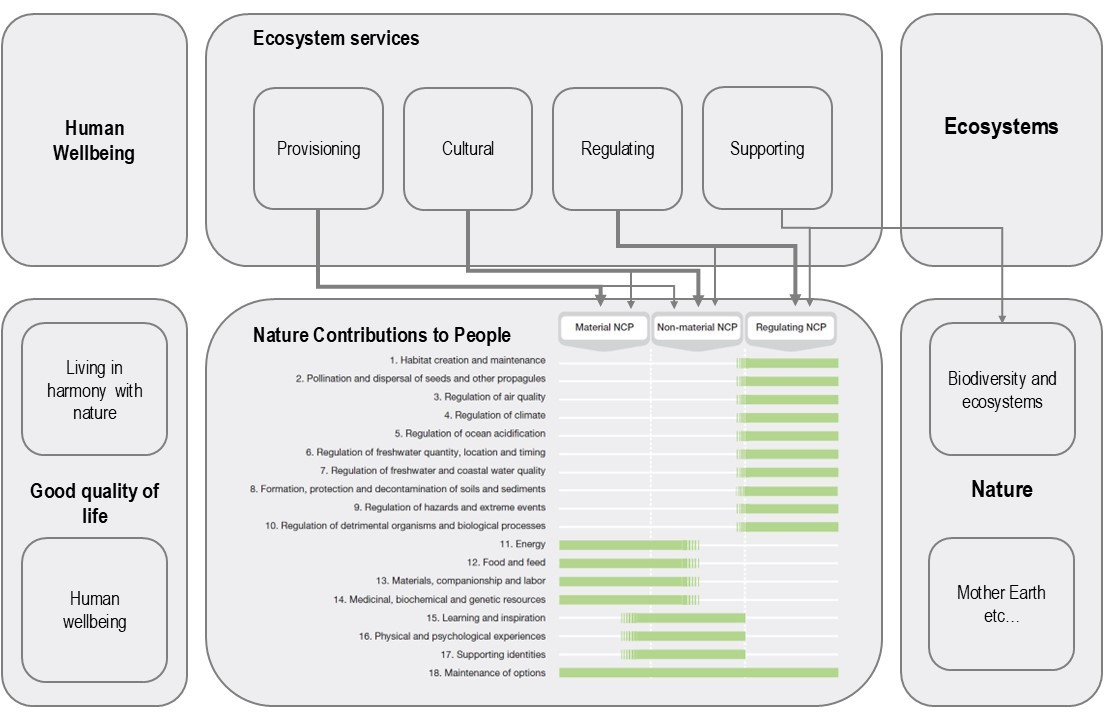
\includegraphics[width = \textwidth]{figures/intro/NCPs2.jpg}
	\caption{Description of the 18 Nature Contribution to People and the connection between the NCP framework \citep{ipbes_2022_6417333} and the Ecosystem Services Framework \citep{millennium2005ecosystems}}
	\subcaption*{Adapted from \cite{diaz_2018} and \cite{ipbes_2022_6417333}}
\end{figure}

Recently, the IPBES platform moved onto a new conceptual framework highlighting Nature Contributions to People (NCP) \citep{DIAZ20151}, defined "all the contributions, positive and negative, of living nature [...] to people's quality of life \citep{diaz_2018}". This framework underpins 3 types of contributions to people: material contributions to people (flows from nature to people typically consumed to "operate a society or enterprise" (IPBES, p.16), non material contributions (eg. nature's effects on "subjective and psychologica aspects underpinning peoples quality of life) and regulating contributions (e.g. "functional and strcutrual aspects of organisms and ecosystems that modify the environmental conditions experienced by people and/or regulate the generation of material and non material contributions"). This framework highlights how Nature Contributions to People can be positive or negative, and depend on the spatial and temporal definition of the contribution, as a given entity can be at the same time the source of positive and negative contributions: for example, forests foster habitat, but also risk endangering people in the event of wildfires. Additionally, it provides a more encompassing view than ecosystem services, as it encompasses perspectives ranging from biodiversity as natural capital employed in an ecological production function (see \cite{polasky_integrating_2009} for a review), as well as perspectives where biodiversity has agency and is linked by reciprocal care obligations to humans \citep{descola}. 


\begin{tcolorbox}[breakable, 
colback=verylightgray, 
colframe=gray!75!black, 
title= {Box 1 - Weak v. Strong Sustainability},
%code={\singlespacing},
fontupper=\small]
\par % This \par ensures spacing before the text starts
\justifying % Start justified text

In 1987, the release of the Brundtland Report \citep{brundtland} provided a broad definition of sustainable development: 

\begin{displayquote}
\textit{"In essence, sustainable development is a process of change in which the exploitation of
resources, the direction of investments, the orientation of technological development; and institutional change are all in harmony and enhance both current and future potential to meet human needs and aspirations"}\\
\small{\cite{brundtland}, p.43}
\end{displayquote}

Implemeting sustainable development remained an open question. In economics, a "weak sustainability perspective", pioneered by works of \cite{hartwick_intergenerational_1977} and \cite{solow_intergenerational_1986} on exhaustible resources, suggested that "maintaining a non-declining capital stock,which allegedly could be put into practice by investing in manufactured capital all the rents derived from the exploitation of non-renewable natural resources" \citep{gomez_history_2010}. In this approach, natural capital could be integrally substituted by human made capital. On the other hand, the "strong sustainability" approach advocates advocates for a complementarity, rather than substitutability of resources \citep{costanza_daly}, acknowledging the dependence of humans on ecosystems
\end{tcolorbox}

This first section highlights a multifaceted correspondence between the different components and dimensions of biodiversity and its contributions to people. Different scales and dimensions of biodiversity underpin NCPs, essential to human livelihood. The global decline of biodiversity threatens NCPs, calling for policy.


%In this dissertation, I narrow the focus on the evolution of single species populations and on the evolution of communities  within a given ecosystem. Moreover, I study the importance of structural diversity at the species and community levels, and focus on animal species. Additionally, I chose to focus on a restricted subset of Nature Contributions to people, within material and regulating NCPs. 

\subsection*{The Importance of Biodiversity and the Challenges of Conservation}
\addcontentsline{toc}{section}{The Importance of Biodiversity and the Challenges of Conservation}

The changes highlighted are of anthropogenic origin with differentiated responsibilities. They emerge from common and specific challenges, which warrant global and local policies. As a wealth of policies are in place, a critical appraisal of their performances is necessary to improve their efficiency.


\subsection*{Anthropogenic drivers of biodiversity decline}
\addcontentsline{toc}{section}{Anthropogenic drivers of biodiversity decline}

The drivers of biodiversity decline are of anthropogenic source. They can be classified between \textit{direct} drivers, e.g. that directly flow form human actions, such as land use change, anthropogenic climate change, overexploitation, and \textit{indirect} drivers, that can be viewed as the root cause for direct drivers, such as  , changes in the value systems that underpin nature uses (\cite{ipbes_2022_6417333} p.55), demography (urbanization and migration), technology, economy (sectoral transitions, trade expansion) and governance (including risht systems for access to resources).

%The Essential Biodiversity Variables framework \citep{pereira_essential_2013} aggregates fine gridded spatial data into 
A synthesis of natural sciences performed by \cite{ipbes_2022_6417333} outlines the roles of principal drivers at the global scale and across realms (see figure \ref{fig:intro_impacts}).
It shows that land and sea use, reefering to the loss, fragmentation\footnote{Undoubtedly, habitat loss is the main driver of terrestrial biodiversity decline. The effects of fragmentation on biodiversity are highly debated. From a theoretical perspective, models have been developed to study the evolution of populations and communities through space and time, e.g. metapopulation and metacommunity models. Theoretical insights highlight that habitat fragmentation increase the extinction risk, and lower colonization probability, resulting in lower survival and diversity \citep{adler_persistence_1994,hill_habitat_1999, thompson_loss_2017}. At the community scale, increases in diversity among communities (e.g. beta diversity) can emerge from different species resource requirements and the larger spatial extent, hence encompassing more environmental heterogeneity, that results from fragmentation \citep{lasky_reserve_2013, chisholm_species_2018}. However, these effects dampen as habitat loss decreases.  
However, at the empirical level, the effect of fragmentation is highly debated. According to \cite{fahrig_ecological_2017}, there is no empirical evidence that a group of small habitat patches generally has lower evological value than large patches of the same total area. Evidence is however found to show that fragmentation does not reduce habitat connectivity, as functional connectivity is improved (e.g. species are in contact with more different resource patches, thus improving the overall functionning). The debate between \citep{fletcher_is_2018} and \citep{fahrig_habitat_2019} surrounds critics based on the ability of statistical models to encompass the effect of fragmentation when habitat loss is present \citep{ruffell_accounting_2016}. Moreover, it reflects the difficulty of landscape ecology, as different mechanisms across scales e.g. patch, landscape and study region, and measures, such as patch size, patch isolation (e.g. distance across patches) and distance to patch edge (e.g. distance to edge within the patch) interact with possible non-linear interactions.}
%
 and degradation of wildlife habitat are responsible for 30\% of the impacts on biodiversity. The direct exploitation of wildlife, wild plants and trees represents 23\% of impacts. Climate change, through shifts in biogeographic conditions and changes in habit, impacts on species traits and genetic evolution represents 14\%, and pollution represents 14\% of impacts. Finally invasive alien species represent 11\%. These drivers have differenciated impacts across ecosystems and biomes \citep{ipbes_2022_6417333}. 

\begin{figure}
	\centering
	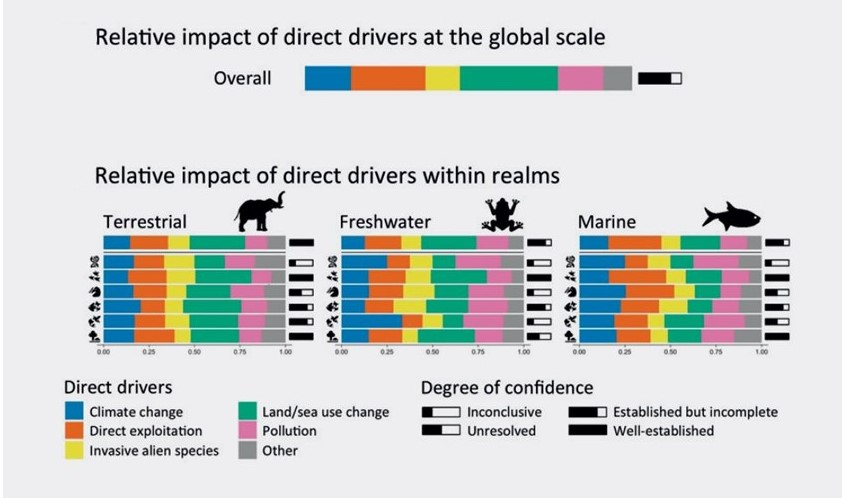
\includegraphics[width = .95 \textwidth]{figures/intro/intro_impactsfin.jpg}
	\caption{Aggregate and realms specific impacts of anthropogenic direct drivers of biodiversity decline adapted from \citep{ipbes_2022_6417333}}
\end{figure}
% Forests
For terrestrial species, land use change is the most important driver (30.5\%), driven by deforestation and agriculture, and direct exploitation follows next (21\%). Tropical and subtropical dry and humid forest host the greatest biological diversity. For example, they host the 10 hotspots with the greatest total number of vertebrates \citep{mittermeier_global_2011}. In such forests, habitat loss and degradation are the main drivers of reductions in species abundance and richness \citep{newbold_global_2014}. Legal and illegal selective logging destroy habitat \citep{hoare2022establishing,  bousfield_2023_large} and are combined with hunting and poaching of wildlife \citep{gallego_2020_combined}, generating between 60 and 180 billions  \$ USD of revenue \citep{gfi_2017}\footnote{Illegal wildlife trade represents between 5 and 23 billion \$USD, while illegal logging represents 52 to 157 billion \$USD}. Mediterranean forests, wooldlands and scrubs, covering 4 million km$^2$, are areas of exceptionally high diversity too \citep{Mooney2001, blondel_2010}. 

However, they are faced with a conjunction of threats, including climate change, land-use transformations \citep{newbold_tropical_2020} and wildfires \citep{Dupuy2019ClimateCI}. Indeed, wildfire frequency and severity are expected to increase with global warming, causing important direct and indirect costs to society including destruction of infrastructure and perturbations to economic activity \citep{wang_economic_2021}, smoke related health conditions \citep{burke_wildfire_2023, heft-neal_behavior_2023}, disrupting structural features of ecosystems \citep{Ayars2023} and threatening biological diversity \citep{Wintle2020}.
% Oceans and fish

For marine species, overexploitation is the main driver (29\%) \citep{ipbes_2022_6417333}. With 90 million tons of capture  (and 141 billion \$ USD)  in 2020 \citep{fao_2022_state}, fisheries stock within biologically sustainable levels have decreased to 64.6\% in 2019, from 90\% in 1974\footnote{ In this calculation, all fishery stocks are equally counted, irrespective of their abundance or catch}, driven by overfishing in the Southeast Pacific and the Mediterranean and Black seas. Assessment of fisheries stock and catch management have been proved to improve livelihoods as well as fish stocks globally \citep{melnychuk_2017_fisheries, hilborn_2020_effective}. Nonetheless, illegal, unreported and unregulated (IUU) fishing is a threat to fisheries. Estimates from 15 years ago \citep{agnew_estimating_2009} estimated it represented between 11 and 26 million tonnes of fis with a value of 10 to 23 billion \$ USD. 

Drivers are differentiated across biomes and species. While certain causes, such as anthropogenic climate change, are overarching, identified drivers pose specific challenges that need to be adressed alone, and in conjuction with other drivers. \\

In this dissertation, I chose to focus on 

\subsection*{Challenges to remedying the drivers of decline}
\addcontentsline{toc}{section}{Challenges to remedying the drivers of decline}

The anthropogenic nature of the drivers of biodiversity decline suggest that anthropogenic actions can also remedy this decline, through policy design and implementation. This requires finding the relevant obstacles and challenges for each drivers and set a determinate courses of actions, at different organisational levels (individual, collective, state implemented or supranational governance).

Habitat loss and overexploitation present both common and differentiated challenges. A common identifiable cause is the large opportunity cost of preserving a species habitat, or existence, in the presence of other economic alternatives for land and time, as well as financial constraints. Additionally, habitat loss and overexploitation share a temporal dynamic aspect, where immediate actions have durable consequences, possibly irreversible.

In turn, specific challenges underly habitat loss and fragmentation (see box 3). In terrestrial ecosystems, land bears a variety of phenomena. At the ecosystem scale, in forests for example, multiple uses pertain to multiple agents (who may be the same person): loggers derive value from cutting and selling timber; settlers have an incentive to deforest for agricultural expansion; hikers value pristine natural conditions and opportunities of sightseeing; conservationists may call for limited management of forest to restore natural cycles; for many, forests must be considered further than their direct use value as they bear a spiritual and religious value. Sometimes, these uses can be in conflict (e.g preferences can be heterogeneous), at many levels: deforestation destroys habitat and sacred land; fuel treatment operations reduce wildfire spread and severity, as well as the huge associated loss, but destroy wildlife habitat. At the species level, some species may bring both positive and negative nature contributions to people. For example, species can be labeled "pests" e.g. causing damages on land when their population densities reach certain thresholds, such as dear, but bring positive contributions to people otherwise \citep{putman_identifying_2011}. As forests support different Nature's Contribution to People, habitat loss and fragmentation is aggravated by climate change, as the distribution of suitable habitat is changed, and phenomena threatening habitats as well as human assets are more frequent and devastating, such as wildfires \citep{Dupuy2019ClimateCI,wasserman_climate_2023}
\\
A second key feature to halt habitat fragmentation is considering the integral set of interdependencies, ecological spillovers and economic externalities that underlie the spatial dimension. The configuration of space, and species movement is at least partly the result of an economic decision. Maintaining habitat connectivity involves identifying patches and paths to be conserved or restored that contribute most to it, in the form of corridors, ecoducts or stepping stones \citep{Turner2005, Turner2011}. The value of patches and paths for connectivity is intrinsically linked to their surrounding : at the same geographic location, a patch has differential value for biodiversity habitat if it is connected to others, or if it is isolated (see box 3). When paths are beyond human control, patches have different importance based on their location, and when the location of patches is fixed, the extent of paths and their location is paramount.
\\
Third, as multiple actions and uses structure connected elements of ecosystems (e.g. different tracts of land, or different biodiversity scales), they trigger spatial spillovers e.g. consequences that go beyond their \textit{in situ} effects. When these spillovers are not taken into account by the agents that generate them, they can be called "dynamic spatial externalities" \citep{sanchirico_bioeconomics_1999, costello_optimal_2008, costello_private_2017}. As halting habitat loss and fragmentation involves conserving tracts of land, neighboring parties may very well benefit (or suffer) from more wildlife and ecosystem (dis-)services on their property, through time. When the a landowner, a community or regional landplanner undertakes fuel reduction operations in a forest, the likelihood of wildfire spreading to their neighbor reduces. These externalities can trigger specific problems of "race to the bottom" \citep{costello_private_2017} : when neighboring parties of a decision maker that undertakes conservation, or risk reduction, fail fail to reciprocate as they benefit from spillovers, a vicious circle of least action is triggered. Conversely, when ecological spillovers are positive, this may lead everybody to use a resource at unsustainable levels \citep{costello_optimal_2008}. Hence, habitat fragmentation and overexploitation are interrelated through spatial connectivity. 
\\
Fourth, improving habitat loss and fragmentation involves coordinating numerous actors towards increasing the area and connectivity of habitat, while taking into account the associated costs and benefits. In some cases, the financial constraints, the magnitude of costs associated with increased habitat connectivity and the difficulty of coordination warrant a public policy where a central planner undertakes the action \citep{Mouysset2012}, but studying decentralized mechanisms, where individuals undertake incentivized actions, are a worth investigating. 
	 
%\textbf{Peut être à bouger dans les politiquess}	 
%	 ; for pests\footnote{For example, the \href{https://www.nrcs.usda.gov/group/143/feral-swine-eradication-and-control-pilot-program}{Feral Swine Eradication and Control Pilot Program} in the US, helped landowners to eradicate feral swines, to restore ecosystems and to change the potential movement of feral swines through landscapes, with fences and traps}, local targeted incentives to control the population and dispersal can have far reaching consequences, if properly targeted. 
	 
	 
%	. As habitat is altered, so is the surrounding matrix, which can impede species movement \citep{eycott_meta-analysis_2012, kuefler_conflicting_2010} and alter evolution and selective regimes \citep{cheptou_adaptation_2017}.  
\clearpage
\begin{tcolorbox}[breakable, 
colback =verylightgray, 
colframe=gray!75!black,
title={Box 2 - Habitat Loss, Fragmentation and Connectivity},
%code={\singlespacing},
fontupper=\small]
\label{box:policy_frameworks_for_biodiv}


\par % This \par ensures spacing before the text starts
\justifying % Start justified text

Habitat loss refers to the loss of areas featuring suitable environmental conditions for species survival and development. At a constant habitat area, fragmentation refers to increases in the number of patches and decrease in the mean size area of each patches, as in figure \ref{fig:connectivity_intro}. \\
Landscape connectivity is defined in relation to fragmentation. It measures "the degree to which the landscape facilitates or impedes movement among resource patches" \citep{taylor_connectivity_1993}. 
It recovers a \textit{structural} dimension, which describes the physical arrangements across patch and a \textit{functional} dimension, which emphasizes the ability and realization of movements of individuals through the landscape.

 Aggregate connectivity measures take into account the role of differentiated patches and paths. In panel D of figure \ref{fig:connectivity_intro}, the circled patch plays an instrumental role in maintaining connectivity. Habitat patch 1 and 2 have the same number of connected patches. However, patch 1 is maintains the connection between the east and west habitat patches in the landscape, and is connected to highly connected patches. Removing habitat patches 1 and 2 would have larger consequences on habitat consequences than removing other identical size patches. Similarly, removing the dotted path (bottom left of panel D) would isolate patch 3, while removing the dashed path would not leave patch 4 isolated. Hence, paths and patches have different impacts on connectivity, depending on the surrounding patches and paths.
\\% Adds some space before the image
\begin{center}
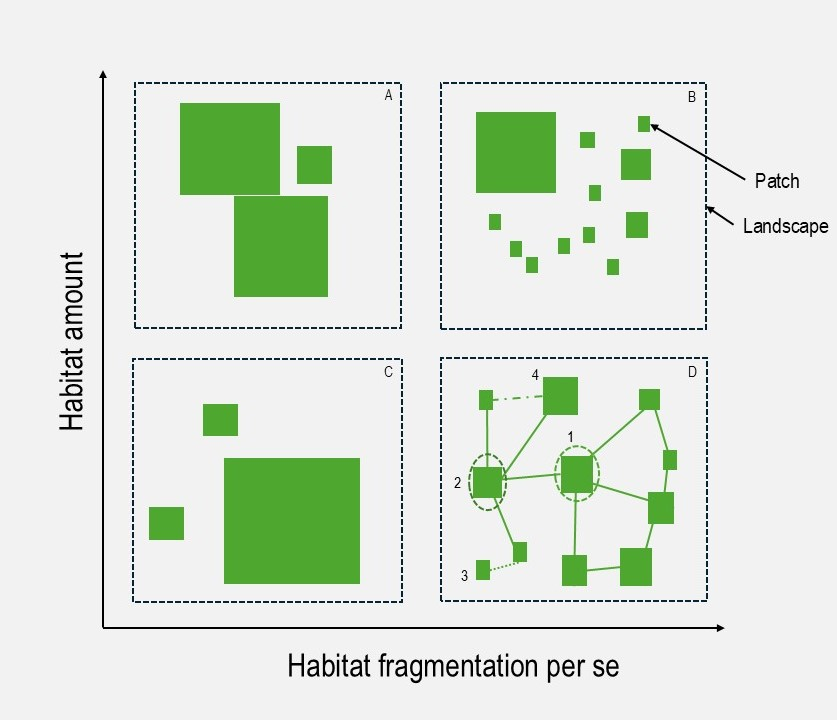
\includegraphics[width = .8\textwidth]{figures/intro/fragmentation.jpg}
\captionof{figure}{Illustration of the effects of habitat loss and fragmentation, adapted from \cite{fahrig_habitat_2019}, and of connectivity}
\label{fig:connectivity_intro}
\end{center}


\end{tcolorbox}

	Halting overexploitation requires understanding and addressing its motives. Overexploitation (or under control, for pests), results from an imbalance between the appropriation and incumbance of Nature's contributions to people (both positive and negative) and the socially desirable level and allocation of these contributions. 	
	The common nature of most natural resources \citep{Gordon1954, smith_models_1969} has long been identified as one of key reason for their demise: numerous events have shown a "race to the bottom", where the absence of secure property rights hastened the overharvest and decline of populations. It has long been the center of attention, and mechanisms to assign property rights have been studied extensively (\textbf{references}). However, while property rights may be assigned, they can be notoriously hard to enforce in areas where regal functions are challenged: \textit{de facto} rights are assigned and enforced. In this case, the common nature of the resource may not be the main concern: local market concentration forces may outweigh overexploitation forces, even in the presence of some of form of open access \citep{damania_economics_2007}. 
Around the world, wildlife poaching and trade typically originates from organised crime groups, and is associated with different criminal activities \citep{mozer_introduction_2023}.  In those cases, concentrated markets tend to emerge and characterize wildlife markets, as competition is hindered by violent organised crime groups. At one extreme, locally monopolistic markets structure for wildlife products may emerge, especially in the case of endemic species (e.g. native and restricted to an area).
They may  be the conservationists' bestfriend \citep{solow_resources_1974, hannesson_note_1983}, depending on specific, context dependent market and species characteristics, as a monopolist has an interest in restricting supply to increase prices, if consumers do not react too much (e.g. under limited demand elasticity). A vast range of  market structures \citep{damania_economics_2007, hannesson_effects_1985} sticking to real world situations have been studied. However, the full range of interactions between a species endemism, local power and harvest structure and access to final consumer markets require more analysis to clarify the impact of market structure.
	Other drivers of overexploitation can be found in the large expected benefits (relative to other local economic activity) some natural resources can bear, most of the time because of their rarity (e.g. absence of economically viable substitute), whether today or in the future \citep{Kremer2000}. While the effects of substituting man-made products to disrupted ecosystem services are starting to get empirically studied \citep{frank_economic_2024} and show how dreadful costs can be, the effect of introducing substitutes to illegally poached wildlife products can be an example of strong substitutability between natural and man-made assets \citep{chen_economics_2017}. As broader forces affect overexploitation, including poverty, it is clear that adressing overexploitation implies generalizing conclusion from the interplay of a single species with the institutional setting, how a  species' future interacts with the availability of substitutes, and how the distribution of revenues from sustainable harvests may foster a reasoned use of the resource. 
	
	A wide range of policies have been implemented at different organisational levels, to jointly or separately halt the identifed drivers of biodiversity decline on land and at sea, with varying degrees of success.


\subsection*{Policies for remedying the decline}
\addcontentsline{toc}{section}{Policies for remedying the decline}

Successive international global policy frameworks have tried to halt ecosystem collapse and biodiversity loss. In 2022, the 15th conference of parties of the UN Convention on Biological Diversity established the \href{https://www.cbd.int/doc/c/e6d3/cd1d/daf663719a03902a9b116c34/cop-15-l-25-en.pdf}{Keunming Montreal Global Biodiversity Framework (GBF)}. This framework replaces the Convention on Biological Diversity's Strategic Plan for Biodiversity 2011-2020 and replaces its Aichi Targets. It sets  four global goals by 2050 and twenty-three measurable targets to halt nature loss by 2030.\\
Goal A focuses on maintaining the ``\textit{integrity, connectivity and resilience of ecoystems}'' such that ``\textit{human induced extinction of known threatened species is halted}",  and on protecting native species abundance and genetic diversity. According to Goal B, in 2050,  ``\textit{biodiversity is sustainably used} and nature contribution to people \citep{DIAZ20151, ipbes_2022_6417333} are ``\textit{valued, maintained and enhanced}''. Finally, Goal C aims at sharing equitably  the uses and benefits from nature, and Goal D that financial means of implementation are secured and fairly and equitably accessible\footnote{See \href{https://www.cbd.int/doc/c/e6d3/cd1d/daf663719a03902a9b116c34/cop-15-l-25-en.pdf}{Section G. Kunming-Montreal Global Goals for 2050}}. Among these goals, several targets are directly geared towards halting habitat loss and overexploitation. Regarding habitat loss, \href{https://www.cbd.int/gbf/targets/2}{target 2} aims to "restore 30\% of all degraded ecosystems" and \href{https://www.cbd.int/gbf/targets/3}{target 3} to "conserve 30\% of land, waters and seas" forming the \textit{"30 by 30" }target. Adressing overexploitation, \href{https://www.cbd.int/gbf/targets/5}{target 5} aims to "ensure sustainable, safe and legal harvesting and trade of wild species", and \href{https://www.cbd.int/gbf/targets/9}{target 9} to "manage wild species sustainably to benefit people"

%\begin{tcolorbox}[breakable, 
%colback=verylightgray, 
%colframe=gray!75!black,
%title={Box 3 - The Convention on Biological Diversity and the Aichi Targets},
%code={\singlespacing},
%fontupper=\small]
%\label{box:policy_frameworks_for_biodiv}
%\par % This \par ensures spacing before the text starts
%\justifying % Start justified text

%In 2010, the Convention on Biological Diversity set its "Strategic Plan for Biodiversity 2011-2020", structured around the 20 Aichi Biodiversity Targets, spanning over 5 goals :

%\begin{itemize}
%\item Goal A : Address the underlying causes of biodiversity loss by mainstreaming biodiversity across government and society
%\item Goal B : Reduce the direct pressures on biodiversity and promote sustainable use
%\item Goal C : To improve the status of biodiversity by safeguarding ecosystems, species and genetic diversity
%\item Goal D : Enhance the benefits to all from biodiversity and ecosystem services
%\item Goal E : Enhance implementation through participatory planning, knowledge management and capacity building
%\end{itemize}

%In 2020, the Global Biodiversity Outlook 5 \citep{global_biodiversity_outlook} showed that none of the Aichi %Target were globally met, and only 6 targets were partially achieved, including the identification and eradication of invasive species on islands, the setting of 17\% of terrestrial and inland water areas and 10\% of coastal and marine areas as conservation areas, the implementation of policy instruments and effective national biodiversity strategy and planning, and the increase in financing biodiversity protection. 

%While several elements showed progress, the failure of the 2011-2020 Strategic Plan was patent. Measurable indicators to assess progress towards targets were missing. This was tackled with the new Global Biodiversity Framework that took over in 2020, although with severe limitations. According to critics \citep{maron_setting_2021}, the current framework also lacks ecological scale-specific indicators (for genes, species, ecosystems) and do not provide specific net outcome statements (such as the 1.5C degree target of the Paris Agreements) across areas, nor a clear implementation timeline. 

%Additionally, the 2011-2020 Strategic Plan failed as countries did not have to report on their progress, only declare their targets. The 2020 Global Biodiversity Framework has implemented follow-up measures : although it is not a legally binding frameworks, countries who have signed commit to demonstrating progress towards the targets and update their National Biodiversity Strategy and Action Plans (see section B.5 and section J of the \href{https://www.cbd.int/doc/decisions/cop-15/cop-15-dec-04-en.pdf}{GBF})
%\end{tcolorbox}

Other international treaties aim at conserving biodiversity, with more delineated action perimeters. Notably, the \href{https://cites.org/fra}{Convention on International Trade in Endangered Species (CITES)} was established in 1973 to regulate and control the trade of endangered species, to halt illegal wildlife trade and ensure species survival. Featuring 183 member parties (countries), it lists species across "appendices", with varying degree of protection of the species and restrictions to trade\footnote{Appendix 1 : the most endangered species, threatened with extinction and prohibited international trade, except when the purpose of exports is not commercial\\
Appendix 2 : species that are not necessarily now threatened with extinction but that may become so unless trade is closely controlled\\
Apppendix 3 : species included at the request of a Party that already regulates trade in the species and that needs the cooperation of other countries to prevent unsustainable or illegal exploitation}. It is a platform to foster international cooperation in enforcing restrictions of trade in protected species.
\\
Restricting the trade in endangered species has debated efficiency. Local enforcement seems to be the key ingredient \citep{HEID2023102784} to recover species, and demand reduction campaings instrumental in achieving species recovery. Additionally, the listing of species may sometimes backfire and increase prices and incentives to poach \citep{hsiang_does_2016}. Yet, for many species, regulatory interventions such as trade bans and controls have failed, and illegal trade in black markets continues to flourish \citep{challender_poaching_2014, challender_towards_2015}. In such instances, supply-side interventions such as conservation farming can theoretically bolster conservation by “flooding the market” with farmed products, leading to reduced market prices and lower poaching incentives \citep{gentry_looking_2019, phelps_framework_2014, tensen_under_2016}. Supply-side interventions have occasionally succeeded at reducing poaching and recovering wild populations – e.g., vicuña and spotted cat \citep{iucn_world_2000, sahley_biological_2007} – but they have also failed – e.g., green python, African elephant \citep{lyons_wildlife_2011, hsiang_does_2016}. Uncertainty around conservation outcomes from market-based approaches has led to continued reliance on trade bans and controls that are often ineffective at reducing poaching.\\

At the national and supranational scales, large scale conservation policies have been implemented, using protected areas. These policies aim at protecting habitat to foster population recovery, as well as mitigating climate change effects on the distribution of suitable habitat. \\
In the United States, in the wake of the environmental conservation/preservation debate \citep{Banzhaf2019}, National Parks have been instated (with the Yellowstone National Park in 1872, and others quickly followed with the creation of the National Park Service in 1916), and followed by other administrative designation restricting the use of land to protect nature and biodiversity, such as the \href{https://www.fs.usda.gov/Internet/FSE_DOCUMENTS/fseprd645666.pdf}{Wilderness Act of 1964}, creating the notion of "wilderness" area where only scientific and non-recreational activities are permitted (for example, motorized vehicles are prohibited). In the wake of the environmentalist movement of the 1960s and 1970s, landmark regulations aimed at protecting natural habitats, such as the \href{https://www.epa.gov/laws-regulations/summary-clean-water-act}{Clean Water Act of 1972} (ensuring sewage to limit the disruption of wildlife habitat), and specifically targeted towards species conservation with the \href{https://www.fws.gov/sites/default/files/documents/endangered-species-act-accessible.pdf}{Endangered Species Act of 1973}. Under this Act, endangered species are listed and actions that directly or indirectly affect them are prohibited, e.g. direct killing or critical habitat modification. Results of the Endangered Species Act are debated. While the impacts seem to be overall positive on species recovery, budget dedicated to listings are slim , and the associated costs are substantial and concentrated on private landowners while benefits are more broadly distributed \citep{brown_economics_1998, langpap_economics_2018}. More localized policies and initiatives, such as the \href{https://y2y.net/}{Yellowstone Yukon Conservation Initiative} (1993), protect and connect ecological areas from Western United States to Canada, using a wide range of tools ranging from local policy-making to working with private landowners to conserve land or design corridors (e.g. connecting areas between ecological areas) between conservation areas.
\\
In Europe and France, habitat policies such as Natura 2000 designed a system of protected areas, established in application of the European Union Birds Directive (1976) and Habitats Directive (1992), and formally in place starting the mid 2000s. In broad strokes, it delineates conservation areas of ecological interest where development and human activities are restricted. Its ambition stemmed from taking into account the scale of biodiversity processes rather than administrative boundaries to develop an interconnected network of conservation areas. To date, the Natura 2000 network is the largest conservation network in the world, spanning close to 28,000 areas and 1,333 000 km$^2$ (e.g. approximately 18\% of land and 9\% of marine areas in the European Union). The ecological and economic performances of such a network are substantial, as they generate spatial spillovers both in terms of economic and ecological performance \citep{cocco_relaxing_2023}. Acknowledging that biodiversity habitat can be seen as a continuum between unsuitable and suitable conditions, mechanisms such as Payments for Ecosystem Services (PES) are leveraged to incentivize conservation on agricultural land. Taking into account the ecological spillovers of decreased spillovers, payments for ecosystem services with agglomeration bonuses, such that neighbors gain an additional marginal benefit when a new local participant implements conservation measures, can be efficient \citep{parkhurst2002agglomeration, bareille_agglomeration_2023}. Overall, the spatial consequences of decentralized policies has yet to be fully integrated in policy making.
\\

Finally, some policies aim at mitigating the threats posed by climate change on ecosystems and species, by changing landscape connectivity. In landscapes where the same surface bears both potential damages and ecological benefits, such as Mediterranean forests, where biodiversity is exceptionally high but wildfires are an ever growing threat \citep{Dupuy2019ClimateCI, wasserman_climate_2023}, fuel treatment operations limit the occurence and severity of wildfires.  Mechanical thinning, prescribed burns, and sometimes, logging, have been leveraged to decrease the fuel load in risky areas and theoretically decrease the probability and severity of burns upon wildfire occurence. In numerous regions, such as conifer forests in California \citep{Vaillant2009, Kalies2016, low_shaded_2023}, eucalypt forests in South Western Australia \citep{burrows2013, boer_long-term_2009, Florec2020}, southern Europe \citep{Fernandes2013}, evidence shows that fuel treatments, can mitigate wildfire intensity and spread. Land management agencies have historically implemented these policies in Australia \citep{burrows2013}, Europe, and the United States (and are projected to ramp up, for example under the Infrastructure Investment and Jobs Act of 2021 in the US). Public policy is leveraged in the face of increasing risk, limited insurability and threats to biodiversity. For example, with limited insurability of homes in the wildland urban interface in California\footnote{For example, \href{https://www.washingtonpost.com/climate-environment/2024/08/29/california-insurance-wildfires-allstate/}{200,000 homeowners will see an increase in their insurance premium} by an average of 34.1\% from Allstate insurance in November 2024. In 2023, the FAIR plan, designed to be the insurer of last resort in California (state mandated but privately funded) saw a \href{https://www.cfpnet.com/key-statistics-data/}{38.3\% increase in its total exposure.}}, as well as the potential economy-wide human and non-human damages from wildfires \citep{wang_economic_2021, heft-neal_behavior_2023, Ayars2023} state-mandated and operated fuel treatment policies are of the essence. However, with increased budgets and improved spatial planning, these policies could achieve better performances in reducing risk while protecting biodiversity.\\
Decentralized policy mechanisms exist, such as mandates to create a defensible buffer around individual properties : in California, a 100-foot defensible around houses is mandates in State Responsibility Areas;  in France, in dedicated regions, the "obligation de débroussaillement" mandates fuel control operations in a 50m radius to "decrease the intensity of wildfires and limit their spread"
\footnote{Translated by the author - \href{https://www.legifrance.gouv.fr/codes/article_lc/LEGIARTI000047809197}{Article L131-10} of the Code Forestier} with fines reaching $5,000$ euros for failing to comply.


I focus on the analysis of the interplay between biodiversity and human actions, through the NCPs it provides and the anthropogenic drivers of its decline. As existing policies have had varying degrees of success in halting biodiversity decline, a framework for policy design is required. I use \textit{economics} to jointly analyze the causes of this decline and offer policy recommendations. 

\subsection*{From the economy to the economics of biodiversity}
\addcontentsline{toc}{section}{From the economy to the economics of biodiversity}

Biodiversity, through its many components, has gradually become an economic object, included both in \textit{the economy} and in \textit{economics}

\subsection*{Biodiversity as an economic object}
\addcontentsline{toc}{subsection}{Biodiversity as an economic object}

Biodiversity, through its different scales, has a longstanding history as an economic object : hunting, fishing, logging have always been instrumental in human livelihoods and became economic objects to be traded. A long tradition has analyzed the specific markets for so-called renewable resources, e.g. whose natural rate of regeneration is commensurable with human experience, as products with an established market price. In doing so, it only considered said resources through a particular ontological state : dead. Focusing on a single species, this approach was only able to elicit the part of the "use value" of species (see \cite{Krutilla1967} and in the modern NCP framework, the material NCPs associated with food and materials) and not the integral value of species \citep{Krutilla1967}. The notion of "use value" had to be broadened to encompass the direct and indirect contributions of species, through a variety of techniques, and put a monetary value on them. To put a price on biodiversity, a wealth of research has relied on market proxies. On the one hand, hedonic methods \citep{rosen_hedonic_1974} have used the variation in observed market prices for a variety of goods, such as real estate, related to the variation of environmental and biodiversity features, and have studied how these variations have been internalized in goods market prices. On the other hand, methods such as the travel cost method \citep{clawson_economics_1967, bhandari_willingness_2010} have relied on observed consumer behavior and expenditures to experience "Nature", such as wildlife seeing, to elicit the price people are willing to pay for biodiversity. When impossible to apply, for lack of proxy or data, other methods have relied on non-market valuation techniques \citep{carson_contingent_2012}. For example, in 1989, the tanker Exxon-Valdez spilled close to 42 million liters of oil in Alaska, in an ecologically sensitive area : marine populations were decimated\footnote{According to \href{https://darrp.noaa.gov/oil-spills/exxon-valdez}{the National Oceanic and Atmospheric Administration}, an estimated 250,000 seabirds were killed, 2,800 sea otters, 22 killer whales, billions of salmons were killed. Numerous species are not in recovery after 25 years}. In order to hold Exxon accountable, surveys were developped to assess the value of marine biodiversity, by surveying the willingness of people to pay for wildlife\citep{carson_contingent_1992, arrow_report_1993, carson_contingent_2003}, with controversed success \citep{Diamond94}. This strand of work pinnacled with \cite{Costanza1997}. In recent years, these approaches have been further developed by departing from direct monetary metrics, towards measuring the influence of species on other outcomes such as health \citep{frank_social_nodate,frank_economic_2024}. Overall, a variety of methods has been leveraged to extend the valuation of biodiversity at different scales, ranging from genetics to habitats, and encompassing functions \citep{bartkowski_capturing_2015}

With the recognition of its economic value, biodiversity indeed became an economic object, which can be subject to direct monetary valuation, although it raises critics. However, this is not sufficient for biodiveristy and its components to become an actual economic\textbf{s} object. While a definition of economics is made difficult with the recent extension of its objects and methods, it is overall concerned with the analysis of human behavior, at the individual and collective level, to manage scarce resources \citep{mankiw_principles_2011, bade_foundations_2002,backhouse_retrospectives_2009}.\\
Key elements in this defnition are \textit{management}, \textit{resource }and \textit{scarcity}. As management requires a commensurability of objects in terms of values (not necessarily with the same indicators, but a basis for rational comparison), it involves weighing opportunities pertaining to different allocations of a resource, as the available amounts are limited e.g. scarce. In the case of biodiversity, at all scales and across types, this implies considering a specific scarcity, as regeneration rates are commensurable with human experience, and potentially, depletion rates. From an epistemological standpoint, this implies considering the temporal dimension of the resource. Hence, while valuation techniques are a building block in making the economics of biodiversity, an explicit framework to consider the temporal dynamic of biodiversity and the consequences of different actions on its current and future state is paramount. To do so, economists use models : 

\begin{displayquote}
 "\textit{[...] a story with a specified structure. The structure is given by the logical and mathematical for of a set of postulates, the assumptions of the model. The structure forms an unninterpreted system [...]. The theorems that follow from the postulates tell us things about the structure that may not be apparent from an examination of the postulates alone. Although the term 'model' is often applied to a structure alone, we shall use it in another sense. In economists' use of models, there is always an element of interpretation: the model always tells a story}"\\
\hspace*{\fill} \small{\cite{GibbardVarian} p. 4}
\end{displayquote}

As such, models appear as mediators between theory and the real world \citep{morgan_models_2009}. \cite{varenne_epistemologie_2014} furthers this approach and labels models as facilitators, across multiple dimensions. A non-exhaustive typology of the roles models can play includes (i) a pedagogical role (facilitating communication), (ii) a predictive role (facilitating anticipation), (iii) a heuristic role (facilitating the explanation of a mechanism with a few simple interactions), (iv) prescriptive (facilitating the response to a given problem) and (iv) integrative (facilitating exchanges between disciplines). Models used in economics encompass these functions to guide the management and policy of biodiversity. 


\subsection*{Bioeconomic modeling for the study and management of biodiversity}
\addcontentsline{toc}{section}{Bioeconomic modeling for the study and management of biodiversity}

Bioeconomic models \citep{Gordon1954, smith_models_1969, clark_profit_1973} have emerged from joint efforts by economists and ecologists to manage resources accounting for the specific dynamics of biotic elements \citep{Parent_Mouysset_Missemer_Levrel_2024}. Bioeconomic models are analytical tools that jointly model the feedbacks between components of biodiversity in wild or weakly manageed ecosystems and economic activities, at different levels (e.g micro, mezzo and macro levels). 
Historically, the first bioeconomic models have emerged from population ecology and static economic analysis, to study the management of fisheries. The Gordon-Schaeffer model highlights the evolution of a fish population according to different harvest regimes, and aims at maximizing revenues in equilibrium. It distinguishes effort levels between those providing the maximum economic yield from those providing the maximum sustainable yield (e.g. resulting in the largest fish growth), yielding new policy perspectives: as the maximum sustainable yield effort is larger than the maximal economic yield, the policy target should be the former. Aiming for the maximum economic effort would therefore yield larger fish populations and promote economic efficiency. The original model was later extended to account for transitory dynamics and integrate elements from capital theory, focusing on the dynamic allocation of resources through time \citep{smith_models_1969, clark_profit_1973}. 

\begin{itemize}
\item Switch to land : other models focus on agricultural contexts and model the evolution of pests
\item Summary of first chapter:
\begin{itemize}
\item Bring MEY and MSY on land : the harvesting paradigm, swanson etc
\item Other approach : no longer monetize biodiversity and increase spatial granularity
\end{itemize}

\item Outline the evolution of bioeconomic modeling with economic models (e.g. taking into account risk and multiple players, as well as switching from pure optimality to more "positive" approaches) and ecological modeling
\item Gradual evolution of models to fulfill different functions of modeling or be different types of facilitators
\\
Box on ecological modeling : from population ecology to conservation and restoration ecology; change of scales, models integrate more and more spatial heterogeneity etc. 
\end{itemize}

\begin{tcolorbox}[breakable, 
colback=verylightgray, 
colframe=gray!75!black, 
title= {Box 3 - A brief overview of ecological modeling for biodiversity},
%code={\singlespacing},
fontupper=\small]
\par % This \par ensures spacing before the text starts
\justifying %
Ecology is a branch of biology that studies of the relationships between living organisms and their environment. 

While 


\end{tcolorbox}

\subsection*{Specific bioeconomic modeling challenges in the face of anthropogenic drivers}
\addcontentsline{toc}{section}{Specific bioeconomic modeling challenges in the face of anthropogenic drivers}

\begin{itemize}
\item Modelling challenges from the literature : 
\begin{itemize}
\item Integrate space in optimal management and focus on the role of space as an endogenous variable, not just spatial granularity
\item Take into account the full interplay of uncertainties : risk, uncertainty, how decision makers adapt etc. 
\item Operating a switch from population ecology to broader scale approaches that still integrate the dynamics of species, and not just static distributions with niches etc, such as landscape ecology and restoration ecology further
\item Integrate indigenous knowledge and perspecitves
\item Refine the study of intricate (to define more) market dynamics
\end{itemize}
\item Current challenges posed in relation with the challenges outlined in the conceptual part for remedy of overexploitation and habitat loss/fragmentation
\begin{itemize}
\item Integrating space in decision making : 
\begin{itemize}
\item deal with non convexity of objective function; 
\item Optimization on discrete landscapes : cannot use continuity
\item Dimensionality curse : dynamic programming fails, at least when performed brutely, so need to trade (i) temporal depth of planning, (ii) extent of space and (iii) complexitiy of ecological mechanisms. 
\item 
\end{itemize}
\item Refine the study of dynamics with heterogeneous and strategic players:
\begin{itemize}
\item Integrate more the roles of ecological and economic heterogeneity through land : limited scope for analytical tractability, need to resort to numerical methods
\item Interaction on a same market of different types of actors, with strategic responses : complicated choice variables in terms of game theory, as exploitation and decision over space are related; 
\end{itemize}
\item Need a variety of perspectives for models to be helpful for decision making : integrating both a positive approach (e.g. compare policy scenarios in a second best world) and a normative approach to guide policy. 
\end{itemize}
\end{itemize}

\subsection*{Research questions}
\addcontentsline{toc}{section}{Research questions}

\begin{itemize}
\item Remind the NCPs I'm focusing on :
\begin{itemize}
\item NCP1 - Habitat creation and maintenance : "the formation and continued production, by ecosystems, of ecological conditions necessary or favorable for living beings important to humans"
\item NCP10 - Regulation of organisms detrimental to humans : "regulation, by ecosystems or organisms, of pests, pathogens, predators, competitors, parasites and potentially harmful organisms"
\item NCP13 - Materials and assistance : "production of materials derived from organisms in cultivated or wild ecosystems and direct use of living organisms for decoration, transport, company and labour"
\end{itemize}
 
How can we adress these drivers jointly, as they share common and specific drivers
\item How can we improve bioeconomic mdodeling to improve policy design that focuses on space and market dynamics? 
\begin{itemize}
\item Can we modernize existing tools to adress pressing policy challenges, in the case of CITES
\item Can we bring new tools (graph theory for example) and perspectives to improve management of space overall, especially in the case of conflicting NCPs? 
\item How can we endogenize decisions over the management of space? 
\end{itemize}
\item Remind the scales of biodiversity : how can we integrate the various scales of biodiversity together, and take full advantage of advances in ecology? 
\end{itemize}

\subsection*{Dissertation outline}
\addcontentsline{toc}{section}{Dissertation outline}
\subsubsection*{Thematic divide of the dissertation}

\begin{table}[H]
\centering

\begin{tabular}{c|c|c}
Driver & Habitat loss, fragmentation& Overexploitation \\
       &  and connectivity   & / underharvest \\
\hline
Chapter 2      & \cellcolor{verylightgray}                    &                                \\
\hline
Chapter 3      & \cellcolor{verylightgray}                    & \cellcolor{verylightgray}      \\
\hline
Chapter 4      &                                              & \cellcolor{verylightgray}   \\   
\hline
\end{tabular}
\end{table}


\subsubsection*{Adressing different scale of biodiversity}


\begin{table}[H]
\centering

\begin{tabular}{c|c|c|c}
Driver &  Biodiversity level & Ecology perspective  & Unit of analysis \\
\hline
Chapter 2      &  Community         &             Landscape ecology                   & Spatial \\
\hline
Chapter 3      &  Population        &  Population ecology   \\
               &                    & and landscape ecology & individuals (biomass stock \\
			   & 				   &  metapopulations  &  and spatial flow) \\
\hline
Chapter 4      &      Population    & Population ecology  & individuals (stock)   \\   
\hline
\end{tabular}
\end{table}

\subsubsection*{Using different model functions and focusing on different methodological challenges}

Explain the data v. theory divide
\begin{table}[H]
\centering

\begin{tabular}{c|c|c}
Driver &  Decision prism  & Model use   \\
\hline
Chapter 2      &  Social planner         &   Prescrptive and pedagogical   \\
\hline
Chapter 3      &  Social planner and decentralized &  Illustrative, pedagogical  \\
\hline
Chapter 4      &      Second best    & Prescriptive and? \\   
\hline
\end{tabular}
\end{table}


\begin{table}[H]
\centering

\begin{tabular}{|c|c|c|}
Driver & \textbf{Space} & \textbf{dynamics}\\
\hline
Chapter 2      &            &                 \\
\hline
Chapter 3      &           &        \\
			  &                     &   \\
\hline
Chapter 4      &          &   \\   
\hline
\end{tabular}
\end{table}

%% Global biodiversity decline : why should we care?

%% Conceptual challenges



